\documentclass[tikz]{standalone}

\usepackage{amsmath}
\usepackage{physics}

\usetikzlibrary{arrows.meta,backgrounds,fit,positioning}

\begin{document}
	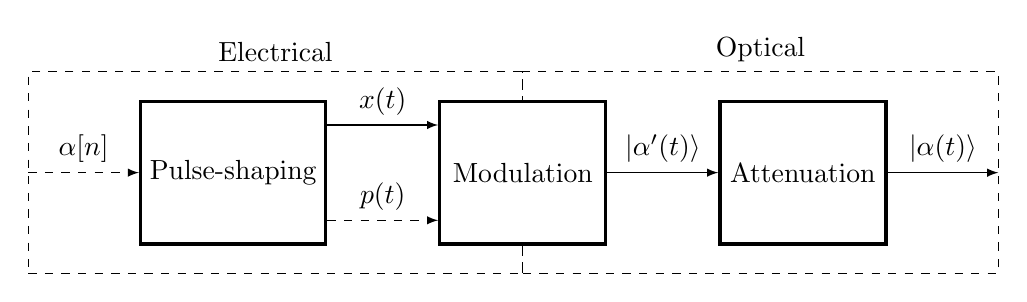
\begin{tikzpicture}[
		node distance=4em,
		arrow/.style={-latex},
		block/.style={draw, very thick, fill=white, minimum height=12ex, minimum width=6em, align=center},
	]
		\coordinate (in) at (0,0);
		\node (psh) [block, right=of in] {Pulse-shaping};
		\node (mod) [block, right=of psh] {Modulation};
		\node (att) [block, right=of mod] {Attenuation};
		\coordinate[right=of att] (out);
				
		\draw[arrow, dashed] (in) -- node[above]{$\alpha[n]$} (psh);
		\draw[arrow] ([yshift=4ex]psh.east) -- node[above]{$x(t)$} ([yshift=4ex]mod.west);
		\draw[arrow, dashed] ([yshift=-4ex]psh.east) -- node[above]{$p(t)$} ([yshift=-4ex]mod.west);
		\draw[arrow] (mod) -- node[above]{$\ket{\alpha^\prime(t)}$} (att);
		\draw[arrow] (att) -- node[above]{$\ket{\alpha(t)}$} (out);

		\begin{scope}[on background layer]
			\node[draw, dashed, fit=(psh.north) (psh.south) (in) (mod.north), label={Electrical}, inner ysep=1em, inner xsep=0pt] {};
			\node[draw, dashed, fit=(att.north) (att.south) (mod.north) (out), label={Optical}, inner ysep=1em, inner xsep=0pt] {};
		\end{scope}
	\end{tikzpicture}
\end{document}
